\chapter{Platoon Combat}
\label{cha:platoon-combat}
% \vfil

\begin{sidebox}{Military Organization}

Organizational units vary from army to army, and from world to world, but it might help to think in terms of the following:

\begin{description}
\item [A team] is composed of 2-5 soldiers of a single vehicle. This is the basic unit of platoon-scale combat, and is represented on the map by a single figure.

\item [A squad] is composed of 1-3 teams and is commanded by a Sergeant or a Corporal.

\item [A platoon] is composed of 2-6 teams, commanded by a Lieutenant.

\item [A company] is composed of 3-5 platoons, under the command of a Captain. This is the largest unit to be controlled by a single player.

\item [A battalion] is composed of 2-6 companies, under the command of a Lieutenant Colonel. An engagement of two battalions is at the extreme upper end of the size of what can be modeled in Platoon-scale combat in Diaspora.
\end{description}
\end{sidebox}
% \vfil


The rules for platoon-scale wargaming are provided in Diaspora for campaigns that want to focus on military combat. Perhaps the players are old army buddies, offering their services to their planet's defense. Perhaps a heavily balkanized world is enlisting off-worlders to fight their battles for them. Perhaps the characters are a mercenary strike team, performing short-term contracts for anyone willing to pay. Whatever the story, it is easy to imagine combats where the scale of personal combat is simply inadequate: when there are too many individuals active in battle, platoon scale provides opportunities for incorporating infantry, artillery, armour and aircraft units in a ground war.

% \vfil

Some campaigns may choose to build around this sort of encounter, with the story effectively moving the characters from one mercenary ticket to the next with each game session. Others might never need these rules, but will be able to occasionally use them to model robbing an armoured vehicle.
%
% \vfil
\iflandscape{\newpage}{}

%
Whatever the application, the rules are provided as a means of representing something that could also be done within the existing Diaspora mechanisms. Operating at the platoon scale becomes an option that is available for those tables that want it.

% \vfil

The organizational unit of interest is the platoon. This is a number of single units, one of which is a leader, all in communication. The only stress track used is the \Morale{} stress track of individual units.

For infantry units, platoon scale represents combat between teams of 2-5 soldiers organized into platoons of 2-6 teams; an armour platoon might be 4 or 5 tanks. Individual characters can improve a platoon's performance, but, as in space combat, an individual can only modify the performance of the larger unit. The principles of FATE still apply, of course, and (as is common in Diaspora), they have been stripped down.

At the platoon scale, there is only a single stress track: \Morale. If a platoon loses morale, it can no longer function. Whether it has lost morale because of its ongoing frustration with lack of supply lines, because of the constant pressure of close enemy fire, or simply because most of the platoon has been killed, Diaspora models the only crucial variable of loss at the platoon scale along the axis of morale.

In most games, players will control either a single platoon, or (as is more usual when used as a stand-alone game) a company of 3-5 platoons.

As with the other mini-games, platoon-scale war-gaming can be played independent of the larger Diaspora RPG.

% \vfil
% \newpage

\section{The Map}\label{sec:social-combat-map}
% \vfil

Social combat takes place on a zone map much as it does with personal combat. Instead of representing some physical geography, the map represents the social space of the encounter. Because of the kinds of options available to characters involved in social combat, certain kinds of map shapes have certain kinds of effects on behaviour and can be used to represent specific issues.

In general, concentric circles imply intimacy. Zone shapes with many borders, and therefore many avenues of escape and access, better represent socially open places like chatting about the weather at a party. Intimate zones are often objectives, such as when you want to get someone to reveal valuable information, and so you want to maneuver them into intimate, trusting conversation.

% \newpage

To begin with, moving between zones has no additional cost --- there is no initial use of ``borders'' as there is in personal combat. Characters in the same zone can be said to be engaging each other socially: they are conversing about interesting, relevant things that they care about. Conversely, the further apart characters are on the map, the more social distance is in their conversation. Range has a deep impact on the effectiveness of characters' interactions and so one must usually close the range before one can do anything useful, such as move the conversation to a more intimate space.

% \newpage

Zones represent in the first instance a degree of intimacy in the social context. This will sometimes correspond to a spatial dimension too, but more often it represents something much more nebulous. For instance, a separate zone might correspond to a small balcony where a conversation might occur. It is often a good idea for the table to design the map of the social combat as a group.

Optionally, once the map is created, each player may choose to place one free-taggable \Aspect{} on a single zone, or a pass value of 2 on a single border, to reflect the personal contours of the social situation.

% badbox here
% \newpage

\subsection{Time}\label{sec:Time}

For each zone on the map, create one time box to represent available time to resolve. If you need to know exactly how long something took, the table should determine the maximum amount of time something is allowed (even the best party will disperse by morning). If a victory condition is achieved before the time boxes run out, the maximum time can be downgraded a number of shifts on the Time Track (Dealing With Time, Chapter 2) equal to the number of unchecked boxes. Often, table consensus will determine a very similar result in any case.

% \newpage

\subsection{The Actors}\label{sec:The Actors}

One of the biggest conceptual hurdles in adopting this system for resolving social interactions is recognizing that not every person in a scene needs to be represented on the map. Part of this is embodied within the zones themselves, as \Aspects{} on the zones can represent the other people involved.

This can in fact be made even more abstract, when you want to make a situation tactical that has become mired or unproductive in regular role-play. By making some of the actors on the map ideas instead of explicit people, you can conduct a scientific investigation or any other information-revealing multi-step endeavour. Make the opposition the Fact and, maybe, an Attractive Falsehood and you can do science. Add in people with conflicting goals (a young whipper-snapper who wants to be primary author on the publication of your discovery!) and the abstract can engage the concrete in both directions.

% \newpage

\subsection{Victory}\label{sec:Victory}

Victory conditions should relate to map position. Usually the objective will be to get a certain person or persons into a specific zone before the timer runs out. This can be more complex, however, to achieve different goals: if you want to model persuading a crowd, you could score participants by how many crowd members are in their target zone when the timer runs out. Feel free to push the system around and find other victory conditions.

\newpage

\subsection{Sample Maps}\label{sec:Sample Maps}

% \newpage

\subsubsection{Party}

A party has a lot of accessible conversation space --- everyone is there to chit-chat after all --- and probably at least one intimate space. It is well represented by a central shape with several attached shapes. Inside one attached space, add a couple of concentric circles for intimacy. An objective in the party might be to hook up with a powerful businessman and get him to brag about his company's secret operation on the dark side of the moon: you win if you can get him, yourself, and the science officer into the center of the intimate zone before the timer runs out.

The party map doesn't need to be complicated --- the simpler it is the faster things will go. The important thing is to make it take a few steps to get to the target zone and be complex enough to imply story with every move. The map above is about the minimum complexity you would want from a social combat map. It might be close to the maximum also!

% \newpage

\subsubsection{Seduction}

\begin{figure}
\centering\footnotesize
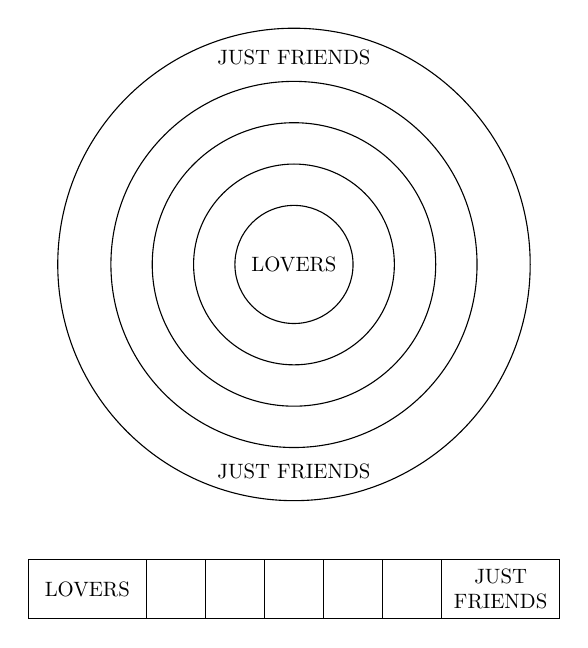
\begin{tikzpicture}[scale=0.75]
\begin{scope}
\draw circle (1) circle (1.7) circle (2.4) circle (3.1) circle (4.0)
  (0,0) node {LOVERS}
  (0,3.5) node {JUST FRIENDS}
  (0,-3.5) node {JUST FRIENDS};
\end{scope}
\begin{scope}[yshift=-5cm]
\draw
  (-2.5,0) rectangle +(-2,-1)
    +(-1,-0.5) node [anchor=center] {LOVERS}
  (2.5,0) rectangle +(2,-1)
    +(1,-0.5) node [text width=1.75cm,text centered] { JUST FRIENDS}
  \foreach \x in {-2.5,...,1.5} {
    (\x,0) rectangle ++(1,-1)
  }
;
\end{scope}
\end{tikzpicture}

\caption{Sample social combat map: Seduction}
\label{fig:social-combat-map-seduction}
\end{figure}

% \newpage


A seduction might be well modeled with a deep set of concentric circles --- say five or six --- with the objective of getting both characters in the bull's-eye (such as in \autoref{fig:social-combat-map-seduction}). Such an engagement could have multiple suitors and possibly require removing some or all from the map through Composure damage.

Suitors might be PCs or they might be NPCs or in some cases they might just be ``pawns'' --- if there is a concept you want to be relevant to the goal but that doesn't necessarily need to have free will in the fight, just give it a marker and no statistics. Players can move it around towards or away from goals (voters in an election or observers at a debate!) but it doesn't do anything on its own.

This could also be done with a simple linear track of, say, seven zones. Mark the first zone \LOVERS{} and the last zone \JUSTFRIENDS{}. Start the seducer on or near \LOVERS{} and the objective on or near \JUSTFRIENDS{}. Start other competitive suitors anywhere that seems fun or scary.

If the objective and anyone else are together on the \LOVERS{} zone, it has fallen for that suitor. If the objective and anyone else are together on the \JUSTFRIENDS{} zone, whoever has joined the objective there is removed from play.

% \newpage

\subsubsection{Debate}

\begin{figure}
\centering\footnotesize
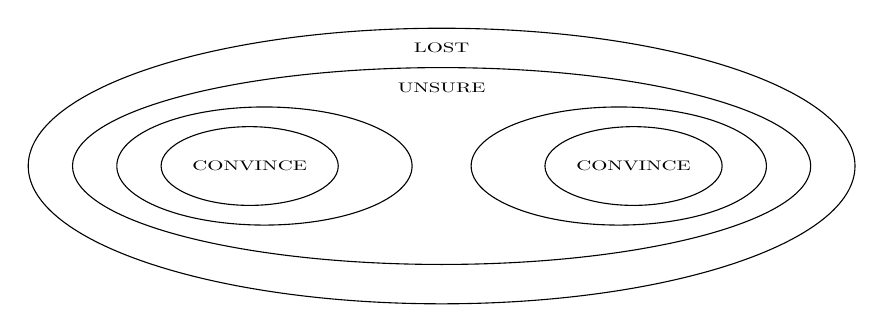
\begin{tikzpicture}[xscale=0.75,yscale=0.5]
\begin{scope}
\draw
  (-3,0) circle (2.5 and 1.5)
  (-3.25,0)   circle (1.5 and 1) node {CONVINCE}
  (0,0) ellipse (7 and 3.5) (0,3) node {LOST}
  (0,0) ellipse (6.25 and 2.5) (0,2) node {UNSURE}
  (3,0) circle (2.5 and 1.5)
  (3.25,0)   circle (1.5 and 1) node {CONVINCE}
%   (-3,0) node {CONVINCE}
%   (0,3.5) node {JUST FRIENDS}
%   (0,-3.5) node {JUST FRIENDS}
;
\end{scope}
% \begin{scope}[yshift=-5cm]
% \draw
%   (-2.5,0) rectangle +(-2,-1)
%     +(-1,-0.5) node [anchor=center] {LOVERS}
%   (2.5,0) rectangle +(2,-1)
%     +(1,-0.5) node [text width=1.75cm,text centered] { JUST FRIENDS}
%   \foreach \x in {-2.5,...,1.5} {
%     (\x,0) rectangle ++(1,-1)
%   }
% ;
% \end{scope}
\end{tikzpicture}

\caption{Sample social combat map: Debate}
\label{fig:social-combat-map-debate}
\end{figure}

% \newpage

A debate can be modeled with two sets of concentric circles representing opposing perspectives (see \autoref{fig:social-combat-map-debate}). The objective would be to move the opponent into your own central circle or moving the majority of audience members into your zone. Note that because of the steep drop-off in effectiveness at range, it will be necessary to move towards your opponent in order to engage him and pull him back to see your point (answering his specific arguments, showing sympathy and understanding).


\section{Command}\label{sec:Command}

\index{command range}
A platoon is a grouping of units that can be ordered to act by a leadership unit. By default that unit must be in the same zone as the leader, but this may be modified by Stunts. The maximum distance allowed between a unit and its leader in order to maintain membership in the platoon is the unit's command range.
%TODO glossary: command range

\rulebox{Command range indicates how may zones a unit can be away from its leader and still be in communication with it.}

\index{OOC|see{Out Of Communication}}\index{Out Of Communication (OOC)}
Command range is zero (same zone only) unless modified by a stunt on the leader, the unit, or both. Non-leader units that do not belong to a platoon (are out of command range) may move away from enemy units, may attack enemy units that have fired upon them, and may attempt to unjam and remove Out Of Communication (\OOC) counters on themselves, but may take no other actions. They have no fate points and do not share a platoon's Consequences. Hits on these units may not be mitigated by a platoon taking a \Consequence. Units that become disassociated from their platoon do not change the platoon's fate point total.

Platoon membership is checked at the beginning of the platoon's action. Units with \OOC{} counters are only part of a platoon membership when in the same zone as the leader unit.

A leader unit with \OOC{} counters disconnects all its platoon members but suffers none of the other restrictions described here.


\section{Units}\label{sec:Units}
\iflandscape{\vfil}{}


A unit is the minimum element represented on the map for each type: a single miniature or counter. For infantry, that's a team of a few soldiers. For armour that's one vehicle. For artillery that's a battery.

There are four types of team units: infantry, artillery, armour, and aircraft. For each platoon, one unit (which may not be aircraft) is also designated the leader. There is no maximum number of units in a platoon.

Each unit in a platoon grants the platoon one fate point. All fate points are kept on the platoon and spent from the platoon. All Consequences are on the platoon.

Similarly, spin counters are associated with platoons and not with units. They may be spent by any unit in the platoon. Spin expires after having had one complete turn in which to use it (thus if spin is acquired during a defensive roll, it lasts until the end of the platoon's next opportunity to act whereas if it is acquired during movement, say, it lasts until the end of the platoons next opportunity to act and not the opportunity in which it moved).

Units that are not normally part of a platoon (typically aircraft) are associated with a particular platoon and donate their fate point to that platoon. They draw fate points from that platoon when invoking, tagging, or compelling.

All units have Skills, Aspects, Stunts, and a \Morale\ stress track. Skills are an n-cap pyramid (i.e. one Skill at level three, two Skills at level two, and three Skills at level one) or a column (i.e. one Skill at level four, one Skill at level three, one Skill at level two, and one Skill at level one).

All units have one Aspect and contribute one fate point to their platoon. Infantry units have a baseline of zero Stunts, plus one Stunt for each technology level. All other units have one Stunt, plus one additional Stunt for each technology level; consequently, units at T-1 or lower do not have Stunts. As described below, the platoon leader always has one additional Stunt, regardless of technology level. No unit may have negative Stunts.

Units have only one stress track: \Morale. When a unit takes a hit past the end of its \Morale\ track that cannot (or will not) be mitigated by a platoon \Consequence, it is eliminated. The narrative associated with this elimination can be determined by the table: it might represent panic and dispersal or surrender; a complete lack of morale is also adequately explained by everyone being killed. Some combination of the three is most likely.  The mechanical effect at this scale is the same. As with other stress tracks, a hit on a marked box rolls up to the next unmarked box.

\subsection{Skills}
\label{sec:platoon-combat-skills}

All Skills are eligible to be chosen by any unit type. See \autoref{tab:platoon-unit-skills} for a list of the unit skills available.

\begin{table}[ht]\centering
\begin{tabular}{lp{0.6\columnwidth}}
\toprule
Skill		& Roll to: \\
\midrule
Anti-air	& inflict harm on aircraft units \\
Armour		& defend against fire \\
Camouflage	& avoid detection \\
Command		& improve (repair) morale \\
Signals		& jam or unjam a unit's communications \\
Direct Fire	& inflict harm in line of sight \\
Hand-to-Hand	& inflict harm in the same zone \\
Indirect Fire	& inflict harm beyond line of sight (including off map) \\
Movement	& move. Without \skill{Movement}, a unit is only capable of advancing a single zone (the free move) per turn. \\
Observation	& detect and locate enemy artillery fire \\
\midrule
Skill		& Description \\
\midrule
Specialist	& sink \Skill\ that has no mechanical effect. The apex \Skill\ of a unit not designed for the represented form of combat (eg, artillery crews as infantry or a staff convoy as armour). \\
Veteran		& modifier to \Morale\ track \\
\bottomrule
\end{tabular}
\caption{Platoon unit skills}
\label{tab:platoon-unit-skills}
\end{table}


Units may only roll Skills for which they are trained. The only
exception is when defending against an opposed roll, in which case the
untrained Skill is presumed to be zero. The only case presented here
is Armour, though with an appropriate Stunt  Camouflage may also
qualify.


% \subsection{Unit Stunts} % should be?
\subsection{Stunts}\label{sec:unit-stunts}
\begin{description}
\item[Cavalry]
this unit is undersized and overpowered, so its maximum move is increased by one (infantry, armour, or artillery only). Infantry units may take this \Stunt\ multiple times: the unit may be thought to have an intrinsic vehicle for mobility. When taken by an armour unit, the \Stunt\ is designated ``\stunt{Light}.''

\item[Special forces]
this unit is not automatically spotted when it shares a zone with an enemy unit (infantry only).

\item[Wireless]
unit is attached to an integrated communications net, increasing command range by 1. May be taken multiple times.

\item[Engineer]
may use a successful maneuver roll to use up the free-tag on an enemy-applied \Aspect\ or make two maneuver rolls on the zone it is in instead of the usual one (infantry and armour only).

\item[Guerrilla tactics]
attacks from this unit never generate spin for the defender (infantry only).

\item[Highly trained]
this unit has one additional morale box.

\item[Infantry carrier]
this unit can carry infantry (armour or aircraft only). One infantry unit in the zone can move with this carrying unit (including traversing the Re-arm track for aircraft). The infantry unit cannot act this turn (before or after the move). The unit can begin the game carrying its infantry load. For aircraft, when the aircraft re-enters the map, the infantry is deployed and may act normally; the aircraft may not otherwise act while deploying infantry. Carried infantry do not have to be in the same platoon as the carrier.

\item[Interceptor]
if this unit is on the LAUNCH! box, it may enter the map any time an enemy aircraft enters the map and act immediately before the target aircraft can act. It may act only against this target aircraft (aircraft only).

\item[Irregulars]
this unit is an irregular non-professional unit (a sink \Stunt, chosen only to model a unit that is less effective than other units of the same technology level). Other sink \Stunts\ can be invented to fit the scenario: \stunt{Slow}, to represent a low rate of fire, etc.

\item[Long range]
ignores one zone for attack roll range modification. May be taken multiple times.

\item[Orbital]
this unit can only be attacked by fire from other orbital units (artillery only). Orbital units that are attacked with the jam action, however, take damage as though attacked with weapons (in addition to the effects of jamming).

\item[Prepared positions]
this unit was set up long before the battle (artillery only). Before combat begins, it may add a the \Aspect\ of \aspect{Locked in} to any two zones on the map. This \Aspect\ can be free-tagged by any allied artillery unit, and remains an \Aspect\ on the zone which may be tagged normally thereafter.

\item[Scatterable mines payload]
this unit can deliver area-denial ordnance (ie, mines). Pass values placed by the unit from an interdiction strike are permanent (artillery and aircraft only).

\item[Scout]
this unit can continue movement after entering a zone containing enemy units (infantry and armour only).

\item[Skill substitution]
With an appropriate narrative, additional \Stunts\ may be designed to allow \Skill\ substitutions. Each unit may only ever have one \Skill\ substitution \Stunt. The following are offered as representative examples.

\begin{description}
\item[Agile]
can use \skill{Movement} in place of \skill{Armour} (armour only).

\item[Graphite payload]
this unit can deliver payloads designed to interrupt electrical and electromagnetic function (artillery and aircraft only).  It may use its \skill{Indirect Fire} Skill to effect Jam attacks (which would normally use the \skill{Signals}). Note that this can be combined with \stunt{Zone Effects} to jam all units in a zone (regardless of owner).

\item[Shoot and scoot]
this weapon system is designed to be fired while on the move or to move very soon after firing a mission. It may use its \skill{Movement} Skill instead of \skill{Camouflage} (artillery only).

\item[Technology enhancement]
increase any \Skill\ by one. This \Stunt\ may be taken at most twice per \Skill, for a total bonus of +2.

\item[Stealth technology]
designed to hide, this unit can use \skill{Camouflage} in place of \skill{Armour} (armour only).
\end{description}

\item[VTOL]
this unit is designed to stay on target --- once on the map it may remain, moving a maximum of 1 zone (its free move) per turn (aircraft only).

\item[Zone effects]
this unit may attack all units in the target zone with one roll at -2 (armour, artillery, or aircraft only). Units do not need to be spotted to be attacked in this fashion.
\end{description}

\subsubsection{Leadership stunts}

Each platoon leader additionally chooses one of the following four Stunts.

\begin{description}
\item [Battlefield genius]
units can be one zone further from the Leader than otherwise allowed.

\item[Logistics genius]
units in platoon do not have the \aspect{Out of ammo} Aspect.

\item[Tactical genius]
units in platoon ignore one extra zone of range when attacking.

\item[Not a genius]
sink Stunt for crap commanders.
\end{description}


\subsection{Stress Tracks}\label{sec:platoon-unit-stress-tracks}

All units have a single stress track, \Morale. A platoon may expend \Consequences to mitigate hits past the end of the track on a unit. A platoon has three \Consequences\ to allocate and each can mitigate two shifts. As is standard in FATE, a platoon \Consequence\ becomes an Aspect and may be free-tagged once or compelled or tagged normally to affect any unit in the platoon.

\begin{itemize}
\item Infantry units have a base \Morale\ stress track of two boxes.
\item Armour units have a base \Morale\ stress track of one box.
\item Artillery units have a base \Morale\ stress track of two boxes.
\item Aircraft units have a base \Morale\ stress track of one box.
\end{itemize}

Unit \Morale\ tracks are modified by the unit's \Veteran\ skill. Leader units also gain a bonus \Morale.

\begin{itemize}
\item Leader units increase the base \Morale\ stress track by two.
\item Units with Veteran 1 or Veteran 2 increase their \Morale\ stress track by one.
\item Units with Veteran 3 or Veteran 4 increase their Morale stress track by two.
\item Units with Veteran 5 or Veteran 6 increase their Morale stress track by three.
\item Some stunts may further alter the length of the Morale stress track.
\end{itemize}


\subsection{Aspects}
\label{sec:platoon-unit-aspects}

All units have one descriptive Aspect chosen by the owner and add one fate point to their platoon. All units also have the Aspect \aspect{Out of ammo}. A unit, when spending fate points, expends platoon fate points. When a unit gains a fate point through a compel, that fate point belongs to the platoon.


\subsection{Infantry}
\label{sec:Infantry}

% \input{C08/TB-infantry}

Infantry units represented a small number of individuals of similar or concerted equipment: a unit typically represents 2-5 individuals, though it could be as many as 12. Specific weapons and armour per individual are not modelled except as they are represented in the Skill and Stunt list.

Infantry have a 3-cap Skill pyramid. Infantry units choose one Skill at rank 3, two Skills at rank 2, and three Skills at rank 1. They have a Morale track two boxes long. If the unit has Veteran at rank 1 or 2, the Morale track is three boxes long. If the unit has Veteran at rank 3, the Morale track is four boxes long.

The maximum movement for infantry is two zones. Infantry units may move a maximum of two zones regardless of their movement roll.


\subsection{Armour}
\label{sec:armour}

Armour units are individual tanks, cars, or other mobile armoured platform. They represent all of the equipment present on precisely that model of vehicle.

Armour has a 4-cap Skill column. Armour units have one Skill at rank 4, one at rank 3, one at rank 2, and one at rank 1. They have a Morale track one box long. If the unit has Veteran Skill 1 or 2, the Morale track is two boxes long. If the unit has Veteran Skill of 3 or 4, the Morale track is three boxes long.

The maximum movement for armour is four zones. Armour units may move a maximum of four zones regardless of their movement roll result.


\subsection{Artillery}
\label{sec:Artillery}

Artillery units are equipment capable of Indirect Fire which are kept off map. They move only in a notional sense insofar as they can roll Movement as a defensive roll against counter-battery detection and Indirect Fire. Infantry-based artillery (such as mortar or grenade launcher crews) should be represented by including an Indirect Fire Skill on an infantry unit. Artillery batteries that need to be represented on the map for purposes of the scenario should be represented by their attending personnel as lightly armed infantry units.

It can be handy to create an off-map artillery card for artillery platoons, especially if they have a command range greater than one. This will greatly simplify aircraft attacks on the artillery platoon. Artillery has a 3-cap Skill column. Artillery units have one Skill at rank 3, one at rank 2, and one at rank 1. Their Morale track is two boxes long. If the unit has Veteran Skill 1 or 2, the Morale track is three boxes long. If the unit has veteran Skill 3, then the Morale track is four boxes long.

Artillery may make Movement rolls to change position on their battery
card if there is more than one zone on the card. Moving artillery
units do not remove \SPOTTED\ markers, however.

Artillery can only fire on targets that are in line-of-sight to a
friendly unit that is currently attached to a platoon (or does not
need to be) and has no Out Of Communications (\OOC) counters.

All artillery units in the same platoon are considered to be in the
same zone as their leader for purposes of command and communication,
and for purposes of any attacks that affect all targets in a single
zone when attacked by aircraft, unless they have a Stunt that allows a
greater command range. All members of an artillery platoon not
situated on the map must be on the same artillery card (they cannot be
spread over multiple cards). Not all units in an artillery platoon
need to actually be artillery units (there might be an infantry leader
unit supplying comms and other coverage and an armour unit supplying
AA for example).
Non-artillery units in an artillery platoon must be in the off-map
artillery card in order to be associated with the platoon. This means
that, although the leader unit might be represented by something other
than artillery (an armour or infantry unit might be more advantageous)
it will gain no advantages from its mobility on the map.


\iflandscape{}{\vfil}
\subsection{Aircraft}
\label{sec:Aircraft}

Aircraft are independent units and therefore require no leader unit. They also move differently from other units: an aircraft unit may place itself on any zone on the map when its turn to act comes up.

Aircraft are automatically spotted when they are on the map.

Aircraft movement is different from other units:

Aircraft begin on the \LAUNCH\ box of the Re-arm track.

While on the Re-arm track, an aircraft unit may make Movement rolls to pro\-gress along the track.

An aircraft on the \LAUNCH\ box at the beginning of its turn may be placed on any zone on the map. Its turn is now over.

Once an aircraft acts while on the map (usually in the turn after it has moved there), it is returned to the RE-ARM box of the Re-arm track.

An aircraft unit on the map may act as any other unit except that it may not make a Movement roll.

Aircraft have a 4-cap Skill column. Aircraft units have one Skill at rank 4, one at rank 3, one at rank 2, and one at rank 1. They have a \Morale\ track one box long. If the unit has \Veteran\ Skill 1 or 2, the \Morale\ track is two boxes long. If the unit has \Veteran\ Skill 3 or 4, then the Morale track is three boxes long.

The maximum movement for aircraft is zero zones as they are not represented on the map. Aircraft units do not move on the map in the same fashion as ground units and so do not make Movement rolls except to decrease their re-arm time.

Aircraft increase range by 1 for all distance calculations (both against them and against other targets).

Aircraft can only be attacked by the Anti-air Skill.


\subsection{Leadership}
\label{sec:Leadership}

Each platoon has one, and only one, leader unit. An infantry, armour, or artillery unit can be designated a leader.

A leader unit may perform a  action in addition to its normal action. It may, therefore, make two  actions in a turn.

Leaders have one Stunt chosen from the leadership Stunts list in addition to the Stunts for their base unit type.

Leaders add two morale boxes to the unit to which they are attached. The maximum movement for leader units is their base unit's maximum movement. Leader units contribute one extra fate point to the platoon (one for the leader and one for the base unit).

Leader units have two Aspects --- one for the leader and one for the base unit --- in addition to \aspect{Out of ammo}.


\subsection{Typical Units}
\label{sec:typical-units}

\input{units/lib-unit-blocks}
\begin{sidebox}{Typical T-1 units}
\centering
\begin{tikzpicture}[scale=0.75]
\tikzstyle{every node}=[transform shape]
\begin{scope}
\infantryblock%
  {Marines}% name
  {B--1}% number
  {they'll never see us comin'}% aspect
  {1/+3/Camouflage,2/+2/Direct Fire,3/+2/Observation,4/+1/Armour,5/+1/Hand-to-hand,6/+1/Command}% skills
  {1/Special Forces/T-1,2/{}/T-2,3/{}/T-3,4/{}/T-4}% stunts
  {}% move
  {4}% morale
\end{scope}
\begin{scope}[yshift=-6cm]
\armourblock%
  {Light Tanks}% name
  {B--2}% number
  {Outfitted for rough terrain}% aspect
  {1/+4/Armour,2/+3/Direct Fire,3/+2/Movement,4/+1/Anti-Air}% skills
  {1/Light/free,2/{}/T-1,3/{}/T-2,4/{}/T-3,5/{}/T-4}% stunts
  {2}% move
  {4}% morale
\end{scope}
\begin{scope}[xshift=6cm,yshift=0cm]
\artilleryblock%
  {Mortar Team}% name
  {B--3}% number
  {Pin-point accuracy}% aspect
  {1/+3/Indirect Fire,2/+2/Camouflage,3/+1/Movement}% skills
  {1/Zone Effects/free,2/{}/T-1,3/{}/T-2,4/{}/T-3,5/{}/T-4}% stunts
  {2}% move
  {4}% morale
\end{scope}
\begin{scope}[xshift=6cm,yshift=-6cm]
\aircraftblock%
  {Bomber Squad}% name
  {B--4}% number
  {Smart-bomb payload}% aspect
  {1/+4/Direct Fire,2/+3/Observation,3/+2/Anti-air,4/+1/Movement}% skills
  {1/Long Range/free,2/{}/T-1,3/{}/T-2,4/{}/T-3,5/{}/T-4}% stunts
  {2}% move
  {4}% morale
\end{scope}
\end{tikzpicture}

% \forlist{\EmptySkill}{\SkillLineNode}{one,two,three}
%   \SkillList(one,two,three)

\end{sidebox}


\vfil

\subsubsection{Typical Infantry}

Skill tree: Camouflage 3, Direct Fire 2, Observation 2, Armour 1, Hand to-Hand 1, Command 1.

Infantry are used to capture and hold territory as well as to provide spotting for heavier units.  They have NCOs capable of regrouping broken units and are adept at close combat as well as ranged. They excel at not being seen.

\subsubsection{Typical Armour}

Skill tree: Armour 4, Direct Fire 3, Movement 2, Anti-air 1.

There are two core types of armour: assault tanks designed to move into heavy fire and attack units spotted by associated infantry, and tank hunters, which would swap Armour and Direct Fire.

\vfil

\subsubsection{Typical Artillery}

Skill tree: Indirect Fire 3, Camouflage 2, Movement 1.

Artillery's immediate objective is to destroy spotted enemy equipment. It does so by projecting a huge volume of fire, which makes it suddenly very vulnerable. It offsets this vulnerability by immediately moving and re-hiding.

\subsubsection{Typical Aircraft}

Skill tree: Direct Fire 4, Observation 3, Anti-air 2, Movement 1.

Aircraft Skill trees are capped by their primary design goal --- Direct Fire for ground attack vehicles, Observation for reconnaissance craft, and Anti-air for interceptors. Most aircraft will be capable in all of these. Movement for aircraft indicates their re-arm time --- high Movement rates indicate rapid re-arming cycles, trading off for specialty effectiveness such as ground attack or anti-air capability.




\section{The Sequence}\label{sec:The Sequence}

Space combat is played in turns, each of which might represent fifteen to thirty minutes of in-game time --- this too has been largely abstracted. Each turn consists of several phases, and each phase will offer a test --- an opportunity to cross-compel, a roll, and an opportunity to tag and/or invoke \Aspects.

\subsection{Detection}
\label{sec:Detection}

% \makeatletter
% \newsavebox{\hbbox}%
% \begin{lrbox}{\hbbox}
% \begin{minipage}[c]{3.8cm}
% \sideboxtitle{Phases}
% The phases are:
% \begin{enumerate}
% \item Detection
% \item Position
% \item Electronic warfare
% \item Beam
% \item Torpedo
% \item Damage control
% \end{enumerate}
% \end{minipage}
% \end{lrbox}
% \begin{wraptable}{r}[\sidebarwidth]{0cm}\end{wraptable}
% \makeatother

% ~

\begin{wraptable}{r}[\sidebarwidth]{5cm}
\centering
% \begin{halfbox}{r}{5cm}{Phases}
\newsavebox{\hbbox}%
\begin{lrbox}{\hbbox}
\begin{minipage}[c]{4.5cm}
\sideboxtitle{Phases of space combat}
% The phases are:
\begin{enumerate}
\item Detection
\item Position
\item Electronic warfare
\item Beam
\item Torpedo
\item Damage control
\end{enumerate}
\end{minipage}
\end{lrbox}
\colorbox{sbbackground}{\usebox{\hbbox}}
% \caption{#5}
% \label{#6}
% \end{halfbox}
\end{wraptable}

Before a fight can start, everyone needs to find each other. Position is plotted on a linear scale from -4 to +4 on the map. As always, before any dice are rolled, the caller will ask for compels, at which time players can compel each other to fail to act. Failure to act in this case is represented by an automatic result of -4 (dice are not rolled and \Skills\ are not considered: your final result for your \Navigation\ check is -4).

A \Navigation\ check is rolled by each ship's navigation officer, and all rolls are ranked. Ties are resolved by raw \Navigation\ \Skill. The highest ranked Navigator will place two of the ships to be played on the map anywhere except the two most distant lines (-4 and 4). The next highest rank then places a single ship and this continues until all ships are placed. The lowest ranking Navigator places nothing. The ship which wins the detection round may also decide if there will be a positioning roll in the first turn (only). Once all the ships are placed, the winning ship in this phase decides whether to proceed to phase 1 or directly to phase 2. This allows a ship to attempt escape without engaging in combat immediately on being detected --- going to phase 1 --- or it allows it to use the tactical position from the detection phase for an optimized initial combat round --- going to phase 2.

In the event of a tie between two ships (as might happen when two standard T2 merchant ships meet, with default navigators), if neither ship is willing or able to invest fate points to gain victory, ships are placed randomly, based on a roll of the fate dice (it is only in this circumstance that a ship may begin at the 4 or -4 band).

\subsection{Position}\label{sec:Position} % \href{sec:id143}

As always, before any dice are rolled, the caller will ask for compels, at which time players can compel each other to fail to act. Failure to act in this case is represented by an automatic result of -4 (dice are not rolled and Skills are not considered: your final result for your positioning check is -4).

Spacecraft positions are plotted on a simple linear scale from -4 to +4. Ships begin as they were placed in the detection phase. At the beginning of each round of combat, pilots jockey for position. All pilots roll their ship's V-shift rating limited by their effective Pilot Skill (i.e. if one character is serving both as Navigator and Pilot, then the Pilot's effective Pilot Skill is reduced by one). Note also that this is not simply a modifier to the roll: since V-shift is limited by effective Pilot Skill, this penalty might affect performance for the first turn as well.

In addition, ships may apply burn: by running their drives over rating, they can exchange Heat for an advantage in maneuver, improving the V-shift roll. Any ship may declare that it is applying burn, state the value and add that value to their roll (not to the V-shift rating). They immediately take a hit to their Heat stress track equal to the value of their burn, marking that box and all unmarked boxes below it. If the highest box to be marked is already marked, mark the next higher open box. Before marking the damage to the Heat stress track, the pilot may reduce the detrimental effects through Consequences exactly as mitigating combat damage. The caller may allow negotiation of burn declarations at his preference, though generally a declared burn rating by a ship's player must stand.

Ships may choose not to use their drives in order to bleed heat. Each turn that the V-Shift is not engaged allows the highest filled box in the Heat track to be cleared immediately. This decision results in an automatic -4 final result for the positioning check, which might still be modified by Aspects, but no dice are rolled and no Skill is used. No burn declarations can be made once the caller declares the bidding closed and asks for dice on the table.

Only the highest roller may alter any ship's positions:
\begin{itemize}
\item He may move himself the difference between his roll and the lowest roll, or
\item He may move any ship with a lower roll up to the level of the
difference between them.
\end{itemize}

He may not, however, move any vessel more map bands than his own vessel's V-shift rating. Remember, moving a ship between the 3 and 4 bar (or the -3 and -4) costs 2 shifts, and moving a ship from the last bar off the map costs 3 shifts.

If the winning positioning roll is tied, the next highest roll is the winner. This presents some interesting tactical choices for fate point expenditure: sometimes it's advantageous to forfeit your awesome roll so that your ally, who rolled lower, can make use of his better V-shift, for example. You might then use an Aspect to force a tie so that you lose control.

If a ship exceeds the band at -4 or 4, they leave combat, whether forced off by others or maneuvered off by their own pilots. In this fashion a really excellent pilot in a hot ship can cut down the odds by positioning enemy vessels off the map until he faces only one opponent. Similarly, more than two ships chasing a single ship can usually keep the lone opponent on the map through positioning.

\subsection{Electronic Warfare}\label{sec:Electronic Warfare}
\vfil
As always, before any dice are rolled, the caller will ask for compels, at which time players can compel each other to fail to act. Failure to act in this case is represented by the ship being unable to declare a target.

Before any destructive weapons are used, each ship may conduct electronic warfare, pitting its communications officer against the enemy. If a communications officer has \stunt{Military-grade Communications}, she may pick a target and roll the ship's \skill{Electronic Warfare} (EW) rating, amplified by her effective \skill{Communications} Skill (if the communications officer has acted in any of the previous phases, there is a cumulative -1 penalty for each phase she has acted). The defender also makes a roll, of his ship's \skill{EW} rating, amplified by the communications officer's effective \skill{Communications} Skill. The rating may be zero, in which case there is there is no crewman staffing the position unless this is done by one of the PCs. Ships may have a Stunt (\stunt{Firewall}) that automatically provides a defense value of 2, and which may not be modified. Subtract the defender's modified roll from the attacker's.

As with any roll, these results can now be modified by tagging or invoking \Aspects\ and paying a fate point to get +2 or re-roll.

Positive values are treated as shifts against the defender, and
%
negative values are treated as shifts against the attacker.
%
Whoever has shifts against him will take a \Data\ stress track hit to the ship. Before damage is calculated, the player may apply \Consequences\ to reduce the number of shifts: a mild Consequence reduces the shifts by one, a moderate Consequence reduces the shifts by two, and a severe Consequence reduces the shifts by four. Recall that no entity can have more than three Consequences of any kind and never more than one of each type.

% \newpage

Once the final number of shifts are determined, the corresponding box on the \Data\ stress track is marked and all open boxes below it are also marked. If the highest box to be marked has already been marked, mark the next highest open box.

Note that only one roll is made for each ship, so in some cases with more than two ships in play, a single roll may defend against multiple attacking rolls as well as conceivably acting as the attacking roll on a declared target. Note also that a good defense against hacking can inflict damage on the attacking \Data\ stress track, even if the defending communications officer does not have Military-grade \skill{Communications}.

The Electronic Warfare (EW) defense roll is persistent through this phase, but the total may be added to over the course of the phase through the spending of fate points. An outnumbered ship may still mount a reasonable defense.

% \newpage

\subsection{Beam Weapons}\label{sec:Beam Weapons} % \href{sec:id145}

Beam weapons subsume all relatively short range unguided weaponry, so they may be described as lasers of various wavelengths, artillery, rockets, railguns, electromagnetically propelled storms of small projectiles, particle beams, or anything else that suits the setting developed at the table. Beams are used both offensively, to directly damage targets at shorter ranges, and defensively, to defend against torpedoes (see Torpedo phase for details).

As always, before any dice are rolled, the caller will ask for compels, at which time players can compel each other to fail to act. Failure to act in this case is represented by a failure to declare a target in whatever phase the player ship was compelled.

A ship with a Beam Skill can attack at any value from 1 up to the full Beam rating. When Beams are fired offensively the attacker must declare what Beam rating he will apply. Note the Beam value used, as it will be relevant in the Torpedo phase.

All combat rolls are made at the Beam rating amplified by the gunner's Gunnery Skill (that is, the Beam rating is used and increased by one if the Gunnery Skill is higher). If the gunnery officer has acted in any of the previous phases, there is a cumulative -1 penalty to the effective Skill level for each phase he has acted. 

Beams firing at three or more bands range subtract 2 from the roll. Attacks are resolved as they are declared, again leveraging social pressure to determine who goes first: the caller closes the call for targets by announcing a final call, and counting slowly to three (if necessary --- if your caller is fair and fun, he'll leave plenty of time), after which no further targets can be announced.

There is no skill to defend against Beams. A roll with no modification is made to oppose all incoming Beam attacks. Ship's may have a Stunt (Vector Randomizer) that changes the base from 0 to 2.
Defensive rolls are made once for each defensive system but stay on the table --- that defensive roll you made against Beams stands throughout the Beam Weapons phase, complete with any modifications from invoking Aspects, using spin, etc. Defensive rolls are persistent through the phase, so it can be handy to note them on the ship card or use a coloured 12- or 20-sided die set to the result. Sometimes we write them on the map. Offensive Beam rolls are distinct from defensive Beam rolls (from the Torpedo phase) and should be recorded separately.

% \newpage

Subtract the defender's final sum from the attacker's to find the number of shifts, and thus the amount of stress on the defender's \Frame\ track. The defender may reduce these by applying one or more Consequences:
\begin{itemize}
\item reduce the shifts by one by applying a mild Consequence
\item reduce the shifts by two by applying a moderate Consequence
\item reduce the shifts by four by applying a severe Consequence.
\end{itemize}

Recall that no entity may have more than three Consequences and never more than one of each kind.

% \newpage

\subsection{Torpedoes}\label{sec:Torpedoes} % \href{sec:id146}

As always, before any dice are rolled, the caller will ask for compels, at which time players can compel each other to fail to act. Failure to act in this case is represented by a failure to declare a target in whatever phase the player ship was compelled.

Torpedoes attack at the spacecraft's Torpedo Skill rating, amplified by the gunner's effective Gunnery Skill (that is, the Torpedo rating is used and increased by one if the effective Gunnery rating is higher). If the gunnery officer has acted in any of the previous phases (including the Beam phase), there is a cumulative -1 penalty for each previously active phase.

Torpedoes firing at one or zero bands range subtract 2 from the roll. Attacks are resolved as they are declared, again leveraging social pressure to build an initiative order as in the Beam phase. The caller closes the call for targets by announcing a final call, and counting slowly to three, after which no further targets can be announced.

A Beam roll is made to oppose all incoming Torpedoes. To do this, the beam position must be staffed. If Beams were fired in the Beam Weapons phase, then the roll may be made as usual, amplified by gunner's effective Gunnery Skill. If Beams were not fired, then there must be a trained crew member available to man the beams in this phase: normal penalties and bonuses apply, but since each crew member may only act once per phase, a ship with a single gunner (as might happen with a skeleton crew) may have to choose between offensive Torpedo fire and defensive Beam fire. Beams so used may also have been fired offensively, and defensive fire may cause damage to the Heat stress track. Ships with no Beam rating or those unwilling to fire Beams defensively, roll with a base of 0 unless they have a Stunt (Point Defense) that changes the base from 0 to 2.

Defensive rolls are made once for each defensive system but stay on the table --- that  defensive roll you made with the Beams stands throughout the Torpedo Phase, complete with any modifications from Aspect invocation, spin, or other sources. As these rolls are persistent through the phase, it can be handy to note them on the ship card or use a coloured 12- or 20-sided die set to the result. Sometimes we write them on the map. Though persistent, defensive rolls are distinct from offensive rolls and should be recorded separately.

% \newpage

When Beams are fired defensively the attacker must declare what Beam rating he will apply. He may apply any value from 0 to the full Beam rating. Note the Beam value used. If the sum of the offensive Beam used in the Beam phase plus the defensive Beam used in the Torpedo phase is greater than the total Beam rating, then the ship takes a hit on the Heat stress track equal to the difference and marks all boxes below as well.

Subtract the final defender's sum from the attacker's to find the number of shifts, and thus the amount of stress on the defender's \Frame\ track. The defender may reduce these by applying one or more Consequences:
\begin{itemize}
\item reduce the shifts by one by applying a mild Consequence
\item reduce the shifts by two by applying a moderate Consequence
\item reduce the shifts by four by applying a severe Consequence.
\end{itemize}

Recall that no entity may have more than three Consequences, nor more than one of each kind.

% \newpage

\subsection{Damage Control}
\label{sec:Damage Control}

Damage control checks may now be made on Frame stress tracks (using one crew member's effective \skill{Engineering} Skill) or Data stress tracks (using one crew member's effective \skill{Computer} Skill). Since each crew may only staff one position per phase, the same individual may not be responsible for both rolls. If the engineer or computer officer has acted in any of the previous phases, there is a cumulative -1 penalty for each previously active phase. The target number for success is the highest box marked on the relevant track. The number of successes indicate the track box that can be erased. Erase it and all unmarked boxes below it.

The Heat stress track cannot be repaired during combat, except by shutting off engines, as described in the positioning phase.


\section{Damage}\label{sec:social-combat-damage}

Stress box hits are not real damage, but they can lead to Consequences. All stress box hits are removed after a few days of relaxing stress-free downtime. As with personal combat, the table should rule when enough time has passed or whether the downtime was sufficiently relaxing. Generally speaking it should be trivial.

\subsection{Recovering Consequences}\label{sec:social-combat-recovering-consequences}

A mild Consequence can be self-medicated with a bottle and some time alone once the scene is over. No roll is required and it is cleared as soon as the social combat scene is over.

A moderate Consequence remains until the end of the session in which it was incurred.

A severe Consequence must be carried through one complete session in which the associated stress track is never marked. If it is incurred during session one, it is gone no sooner than the end of session two, and if the associated stress track takes hit in a fight during that session, you'll need to hold the Consequence through yet another one.


\section{Characters in Platoon Combat}\label{sec:characters-in-platoon-combat}

A character may be associated with any unit. While more than one character can be associated with a single unit, for playability it helps to assign characters to different units, to allow players something to control during the game. A single character stand can have his base touching the associated unit base for representation, but it is easier just to note which character is associated with which unit separately. The player character moves with the unit. If the unit is destroyed, the player character is no longer involved in the combat (he's gone to ground, run off, or dead --- let the player narrate his escape).

Each character associated with a unit may, however, amplify one Skill of the unit. The player may choose which Skill gets amplified based on \autoref{tab:amplifying-platoon-skills}.

\begin{table}[ht]
\centering
\begin{tabular}{ll}
\toprule
Unit Skill	& Amplified by \\
\midrule
Anti-air	& MG Slug Thrower \\
{}		& MG Energy Weapons \\
{}		& Gunnery \\
Armour		& Tactics \\
Camouflage	& Stealth \\
{}		& Survival \\
Command		& Tactics \\
{}		& Intimidation \\
{}		& Oratory \\
Signals		& Communications \\
Direct Fire	& Slug Thrower \\
{}		& Energy Weapons \\
Hand-to-Hand	& Brawling \\
{}		& Close Combat \\
Indirect Fire	& Gunnery \\
{}		& Demolitions \\
Movement	& Tactics \\
{}		& Vehicle \\
Observation	& Alertness \\
Veteran		& Resolve \\
\bottomrule
\end{tabular}
\caption{Amplifying Platoon Skills}
\label{tab:amplifying-platoon-skills}
\end{table}


\section[Wargaming]{Wargaming}
\label{sec:personal-combat-wargaming}

Sometimes it's fun just to make one-off characters and have them shoot at each other. To play independently as a tactical war game, you need three things: a map, a story, and characters.

\subsection{The Map}
\label{sec:personal-combat-wargaming-map}

Someone is chosen as caller. Either the caller or the table draws a map. Is it a shoot out in an airport? A race to secure a bunker at the top of a hill? A boarding action in a submarine or a spaceship? Whatever the case, you need a map to play on.

You can start with a blank piece of paper, and take turns drawing features, until it looks good enough. Feel free to write words on the map too – these can become Aspects and help clarify what's what.

Once that is done, divide the map into zones. You don't want too many, but enough to allow opportunities for getting outside of range, and to allow movement. When drawing zones, it is often helpful to go from corner to corner: that means it is always clear when a character enters an area (from a door, or otherwise along a side) what zone he is in.

\subsection{The Story}
\label{sec:personal-combat-wargaming-story}

The process of drawing a map has already begun to determine what the story is: is this a fight to the death? Are there teams? Is most of the table maneuvering against a small cadre controlled by the caller (or by someone else)? Is there a difference in tech level between two sides? Whatever the case, articulating the story that is being told might mean that you go back and change the map slightly, add an Aspect to a zone or two, or whatever.

Most important is that the story articulates victory conditions, which need not be the same for all players. Is this a fight to the death? An attempt to capture someone alive? Someone working to escape detection and get out of a building, or sabotage a spacecraft's drives? Whatever the case, the victory condition might be defined in terms of time: get off the ship in eight turns; spend two turns alone in the engine room setting explosives.

\subsection{Characters in Wargaming}
\label{sec:characters-in-wargaming}

\iflandscape
{\begin{wraptable}[14]{r}[0.9\sidebarwidth]{5cm}}
{\begin{wraptable}[14]{r}[0.9\sidebarwidth]{5.5cm}}
% \begin{table}[ht]
\centering
\begin{tabular}{ll}\toprule
Skill & type \\
\midrule
Agility		\\
Alertness	\\
Brawling	& combat \\
Close Combat	& combat \\
Energy Weapons	& combat \\
EVA		\\
MicroG		\\
Resolve		& track \\
Slug Throwers	& combat \\
Stamina		& track \\
Stealth		\\
Tactics		\\
\bottomrule
\end{tabular}
\caption{Useful skills for personal combat wargaming}
\label{tab:personal-wargaming-skills}
% \end{table}
\end{wraptable}


Once the map and the story are determined, everyone should spend five minutes (no more) making one or two characters to push around the map.

\subsubsection{Skills}

Given the limited focus of this tactical game, 3-cap characters should be sufficient: pick one Skill at level 3, two at level 2, and three at level 1. Everything else is considered untrained. While any Skill might be taken, \autoref{tab:personal-wargaming-skills} presents Skills particularly relevant to this mini-game.

\subsubsection{Stress Tracks}

Characters should only concern themselves with the \Health{} and \Composure{} stress tracks. Each is three boxes long. If the character has \skill{Resolve} at level 1 or 2, the \Composure{} track has four boxes; if he has \skill{Resolve} 3, the \Composure{} track has five boxes. If the character has \skill{Stamina} at level 1 or 2, the \Health{} track has four boxes; if he has \skill{Stamina} 3, the \Health{} track has five boxes.

\subsubsection{Stunts}

Every character selects a Stunt. Making something Military-grade or altering how a stress track works are both obvious choices. (For some stories, it may be desirable to allow two Stunts per character; that's fine, as long as it's the same across the board).

\subsubsection{Aspects}

Each character should have three Aspects, revealed to all at the table. Each character also begins with three fate points.

Making a note card for each character, placed in front of the player with all the relevant information and a small pile of fate points stacked on top keeps all the information clear at all times. This is obviously scaled back from the RPG, and introduces a slightly different calculus for what constitutes a success. With reduced characters, teamwork, particularly in laying down maneuvers to be free-tagged, is rewarded.

